% https://ask.latexstudio.net/ask/question/17455.html
\documentclass[tikz,border=2pt]{standalone}
\usetikzlibrary{calc,intersections}
\newlength{\bigenough}
\newcount\total
% locates both points on a closed shape tangent to a point outside the shape.
% \tangent{pathname}{center}{point}{first}{second}
\newcommand{\tangent}[5]% #1=path name for shape, #2=coordinate name for center, #3=cordinate name for outside point
{\begingroup% #4=coordinate name for first tangent point, #5=coordinate name for second coordinate point
\setlength{\bigenough}{1cm}
\loop% loop until big enough
  \path[name path=temp]  ($(#2)!\bigenough!-90:(#3)$)--($(#2)!\bigenough!90:(#3)$);
  \path[name intersections={of = #1 and temp, total=\t}]%
    \pgfextra{\global\total=\t};%
  \ifnum\total<2 \global\bigenough=2\bigenough\repeat%
\endgroup
\coordinate (#4) at (intersection-1);% initial guess
\coordinate (#5) at (intersection-2);%
\tangentsearch{#1}{#2}{#3}{#4}%
\tangentsearch{#1}{#2}{#3}{#5}}

% find tangent using binary search
\newcommand{\tangentsearch}[4]% #1=path name for shape, #2=coordinate name for center, #3=cordinate name for outside point
{\begingroup% #4=coordinate name for tangent point (initail guess -> final)
\loop% loop until only 1 intersection
  \path[name path=temp] (#3)--($(#4)!-\bigenough!(#3)$);
  \path[name intersections={of = #1 and temp, total=\t}]%
    \pgfextra{\global\total=\t};%
\ifnum\total=2 \coordinate (#4) at ($(intersection-1)!0.5!(intersection-2)$);
  %\draw[pink] (intersection-1)--(intersection-2);% included only for debugging purposes
  \path[name path=temp] (#4)--($(#4)!-\bigenough!(#2)$);
  \path[name intersections={of = #1 and temp}];%
  \coordinate (#4) at (intersection-1);%
  \repeat%
\endgroup}

\begin{document}
    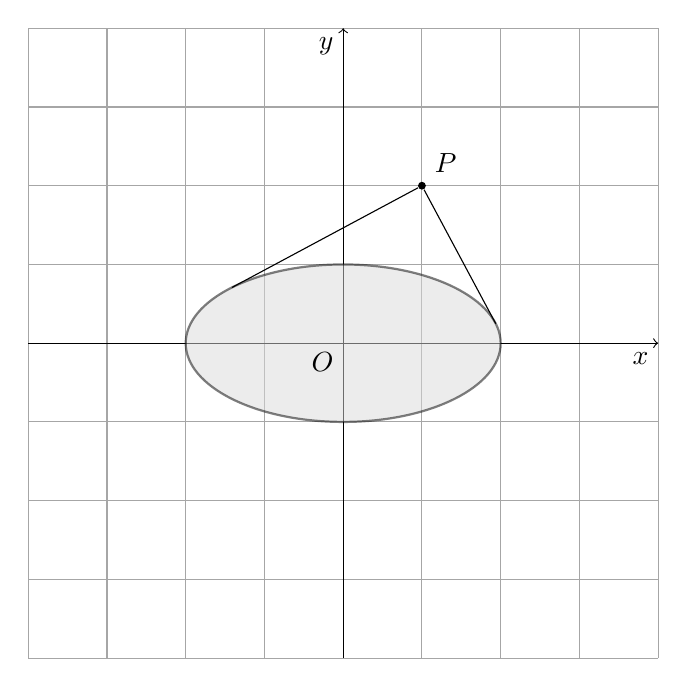
\begin{tikzpicture}
        \draw [gray!70] (-4,-4) grid (4,4);
        \draw [->] (-4,0) -- (4,0) node [below left] {$x$};
        \draw [->] (0,-4) -- (0,4) node [below left] {$y$};
        \draw[name path=ellipse,thick,fill=gray!30,opacity=0.5] (0,0) ellipse (2 and 1);
        % \draw [thick] (2,0) arc (0:360:2 and 1);
        %\coordinate (O) at (0,0);
        %\node at (O) [below left] {$O$};
        %这里可以缩行
        \coordinate[label={below left:$O$}] (O);
        % \coordinate (P) at (1,2);
        % \fill (P) at (1,2) circle (1pt) node [above right] {$P$};
        %这里也可以缩行
        \node[label={above right:$P$},circle, fill, inner sep=1pt] (P) at (1,2) {};
        \tangent{ellipse}{O}{P}{X}{Y}
        \draw (X)--(P)--(Y);
    \end{tikzpicture}
\end{document}